\section{Konfiguration}


\begin{figure}[ht]
  \centering
  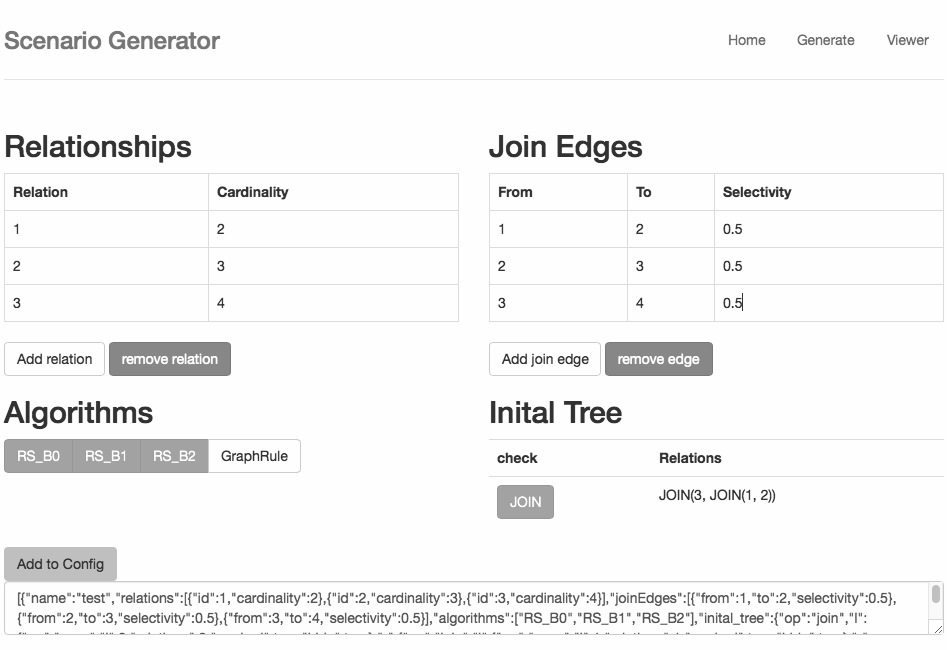
\includegraphics[width=1\textwidth]{04_Implementierung/00_media/Tool.png}
  \caption{Konfigurationstool: Scenario-Generator}
  \label{ScenarioGenerator}
\end{figure}

Das Konfigurationsmodul besteht aus zwei Komponenten. Auf der einen Seite eine Javascript-HTML Anwendung zur Generierung von Test-Szenarien (vgl. Abb. \ref{ScenarioGenerator}). Mit Hilfe dieser Anwendung können Konfigurationsfiles für den späteren Test erstellt werden. Dieses Konfigurationssystem, das in  zu sehen ist, bietet dem Nutzer die Möglichkeit Relationen mit Kardinalitäten zu erzeugen, Selektivitäten festzulegen und schlussendlich einen initialen Plan zu erzeugen. Ebenfalls ist es möglich die verschiedenen Regelmengen, die geprüft werden sollen, festzulegen.

Das Ergebnis dieses Moduls ist eine Konfigurationsdatei im JSON-Format. Das Tool unterstützt die Erzeugung mehrerer Szenarien in einem Konfigurationsfile. So können mehrere Szenarien in einem Test-Run durchgespielt werden. Die Verwendung des JSON-Formats bietet viele Vorteile. U.a. waren die folgenden Vorteile ausschlaggebend für die Verwendung von JSON:

\begin{itemize}
\item Im Gegensatz zu XML ist JSON einfacher. Weniger Grammatik ist vorhanden.
\item Das Format ist hoch interoperable und kann nativ von Javasciript ausgegeben werden. Ebenfalls ist es möglich mit Hilfe von einfachen Parsern JSON in C++ zu verarbeiten.
\item JSON ist durch die einfache, jedoch standardisierte Form leicht für den Menschen zu lesen und Fehler sind leichter aufzuspüren.
\item Das gewählte Format zur Repräsentation der unterschiedlichen Parameter ist einfach erweiterbar. Attribute und neue Objekte können jederzeit hinzugefügt werden.
\end{itemize}

\subsection{Aufbau und Funktion der Konfigurationsdatei}

Ein konkretes Test File ist in \ref{JsonConfigFile} zu sehen. Jedes Test File ist ein Array von Test-Objekten. Für jeden Test wird mit dem Attribut \texttt{name} ein Name gespeichert. Für jede Relation, die in einem Test vorkommt, wird ein Relations-Objekt erzeugt. Es besteht aus einer \texttt{id}, der Relations-Id, und der dazugehörigen Kardinalität. Mehrere dieser Relations-Objekte werden in einem Array gespeichert und sind dem \texttt{relation}-Attribut des Test-Objekts zugewiesen. Im konkreten Fall sind zwei Relationen vorhanden. Eine mit der \texttt{id:1} und eine mit der \texttt{id:2} 2. Für Beide wurde eine Kardinalität zugewiesen. 

Auch für Join-Kanten werden Objekte erzeugt. Ein Join-Kanten Objekt bezeichnet eine Kante zwischen zwei Relationen. Eine Kante könnte, wie im Beispiel zu sehen von der Relation 1 zu der Relation 2 verlaufen, wobei die Richtung nicht entscheidend ist. Einer Join-Kante wird auch eine Selektivität zugeordnet. Mehrere dieser Join-Edge-Objekte werden als Array im Attribut \texttt{joinEdges} hinterlegt.

Neben Join-Kanten und Relationen sind auch die zu testenden Algorithmen gespeichert. Sie werden in einem Array abgelegt und sind dem Attribut \texttt{algorithms} zugewiesen. Im vorliegenden Beispiel werden die Regelsets \texttt{RS-B0}, \texttt{RS-B1} und \texttt{RS-B2} getestet.

Auch ein initialer Plan wird im Test-Objekt gespeichert. Ein Baum besteht immer aus Knoten. Für jeden Knoten wird ein Operator im Attribut \texttt{op} gespeichert. Es wird der Operator \texttt{SCAN} und der Operator \texttt{JOIN} unterstützt. Ein Knoten kann eine linke und eine rechte Seite haben. In Zeile 14 ist eine Scan Operation zu sehen. Es wird nur die linke Seite verwendet. Im Attribut \texttt{l} ist die ID der Relation abgelegt, die zu scannen ist. Bei \texttt{JOINs} wird auch die rechte Seite verwendet (vgl. Zeile 16). In den Attributen \texttt{l} und \texttt{r} können entweder weitere Knoten oder Relations-Ids gespeichert werden. Neben Operator, links und rechts ist das Attribut \texttt{relations} Teil des Knotens. Hier ist eine einfache Repräsentation des Knotens gespeichert. Im Falle von Zeite 14 \texttt{1}. sind komplexere Knoten und Subknoten vorhanden,deshalb  können komplexere Daten im Feld \texttt{Relations} abgelegt sein. Beispielsweise ist eine solche komplexere Form in Zeile 19 ( \texttt{JOIN(1,2)}) zu erkennen. Hier ist ein Join zwischen 1 und 2 zu sehen.

\begin{figure}[ht]
\lstinputlisting{04_Implementierung/00_media/config.json}
\caption{JSON: Konfigurations-File}
\label{JsonConfigFile}
\end{figure}

\subsection{Konfiguration eines Test innerhalb des Prototypen}

Die eigentliche Konfiguration findet in C++ statt. Mit der Bibliothek json11 \cite{json11} wird das Konfigurationsfile gelesen. Dieser Vorgang wird von der Klasse \texttt{Config\-urator} übernommen. Auf Basis eines Dateipfades zu einer Konfigurationsdatei erzeugt die Klasse einen Vektor von \texttt{Configuration} Instanzen. Für jedes JSON Test-Objekt wird eine solche Konfigurationsinstanz erzeugt und die für die Konfiguration notwendigen Informationen hinterlegt.

Jedes Konfigurationsobjekt (vgl. Abb. \ref{Konfiguration}) bietet eine Menge unterschiedlicher Methoden an, um Informationen über den aktuellen Test zu erlangen.

Mit Hilfe der Methode \texttt{getInitaleTree()} wird ein Baum aus Äquivalenzklassen und Planknoten erstellt, die den initialen Plan erzeugen. Die Methode ergibt immer eine neue Instanz des gesamten Baums.

Die Kardinalität und Selektivität, die als ausschlaggebende Kennzahlen zur Berechnung des optimalen Plans herangezogen werden, sind mit den Methoden \texttt{get\-Cardinaility()} und \texttt{get\-Selectivity()} zu erfragen. Auch die getesteten Algorithmen können mit der Methode \texttt{getAlgorithms()} ausgelesen werden.


\begin{figure}[ht]
  \centering
  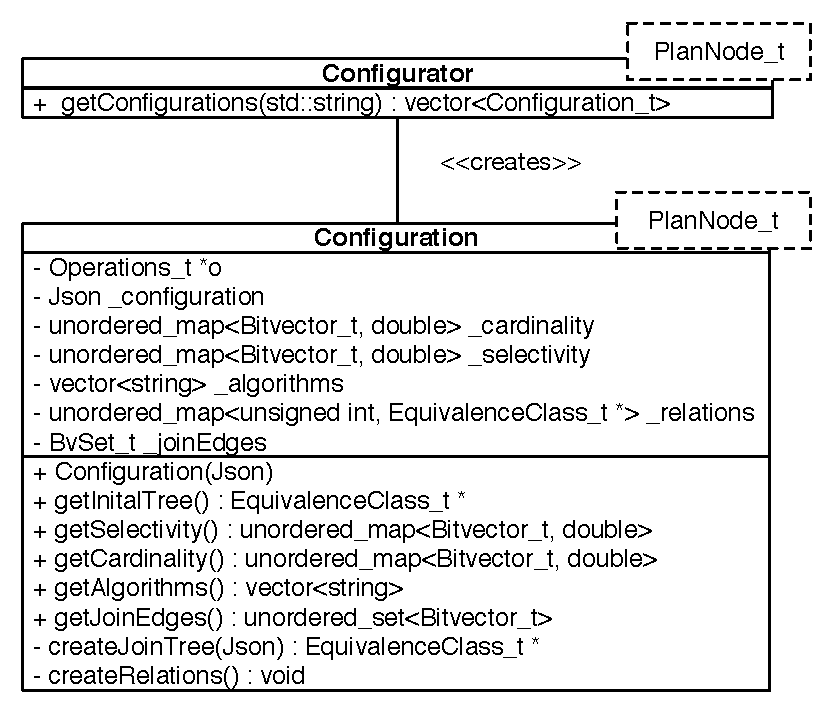
\includegraphics[scale=0.75]{04_Implementierung/00_media/ConfigurationClass.pdf}
  \caption{Klassendiagramm: Konfiguration}
  \label{Konfiguration}
\end{figure}
